\documentclass[letterpaper,12pt]{article}
\usepackage{tabularx} % extra features for tabular environment
\usepackage{amsmath}  % improve math presentation
\usepackage{float}
\usepackage{pdfpages}

\usepackage{graphicx} % takes care of graphic including machinery
\graphicspath{ {./figures/} }
\usepackage[margin=1in,letterpaper]{geometry} % decreases margins
\usepackage{cite} % takes care of citations
\usepackage[final]{hyperref} % adds hyper links inside the generated pdf file
\hypersetup{
	colorlinks=true,       % false: boxed links; true: colored links
	linkcolor=blue,        % color of internal links
	citecolor=blue,        % color of links to bibliography
	filecolor=magenta,     % color of file links
	urlcolor =blue         
}




\begin{document}

\title{Experiment 1 Preliminary Work \protect\\ Diodes and Rectifiers}
\author{Ahmet Akman 2442366 \protect\\}
\date{\today}
\maketitle

%\begin{abstract}
%abstract
%\end{abstract}

\section{Introduction} 
\section{Step 1}
Notes on signal generators, oscilloscopes and multimetersi are studied and reviewed the fundamentals.
\section{Step 2}
Notes on dioedes document is studied. The datasheets of the diodes to be used in this experiment are reviewed, which are \href{https://www.vishay.com/docs/88503/1n4001.pdf}{1N40007} , \href{https://www.vishay.com/docs/88536/ba157.pdf}{BA159} ,\href{https://logosfoundation.org/elektron/mixers/AA119.pdf}{AA119} ,and \href{https://www.vishay.com/docs/85604/bzx55.pdf}{BZX55C-6V2}.   
\section{Step 3}
%MATLAB and Latex
In this step characteristics of linear modeled junction diodes are analyzed according to the I vs V equation as follows,
\[
I  = I_s[e^\frac{qV}{nkT} - 1]    
\] 
Ideality constant n is taken 1 for both cases. From explanation in the manual \(\frac{kT}{q}\) is taken as 25 mV at temperature (20\(\circ\)C ) . The common pievewise linear model for a junction diode is given in Figure 1.
\begin{figure}[H]
    \centering
   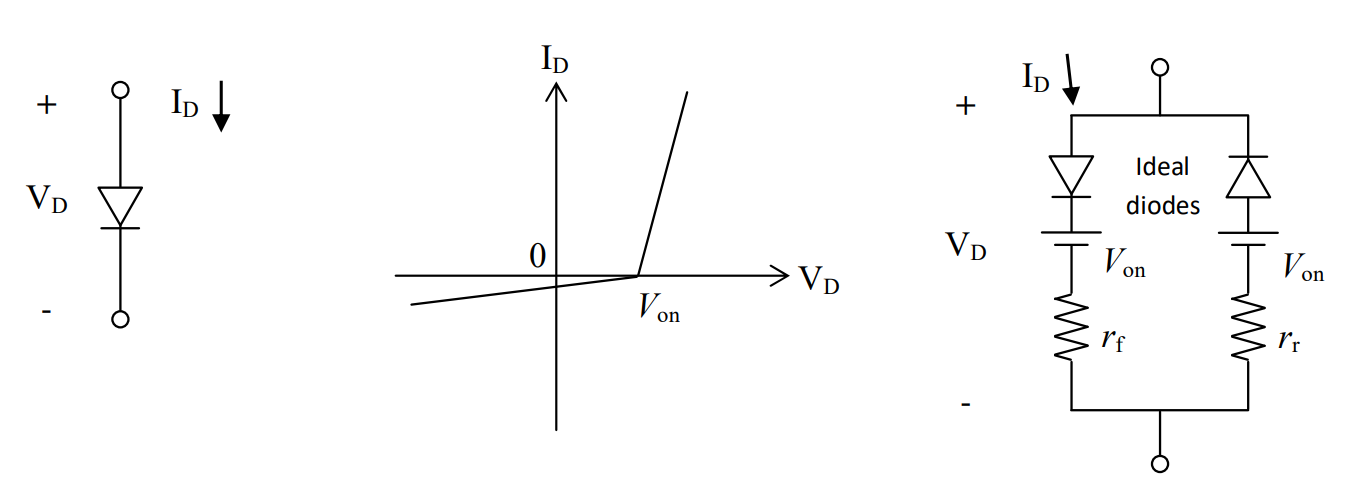
\includegraphics[width=1\textwidth]{3_1.png}
   \caption{Common piecewise linear model for a junction diode.}
\end{figure} 

\subsection{a)}


\begin{table}[H]
\begin{center}
\caption{ I vs V}
\vspace{2mm}
\begin{tabular}{||c | c ||} 
\hline
V(Volts) & I (Amps) \\ [0.5ex] 
\hline\hline
-0.40 & -2.499999718662063e-07  \\ 
\hline
-0.20 & -2.499161343430244e-07  \\ 
\hline
0 & 0  \\ 
\hline
0.10 & 1.339953750828606e-05  \\ 
\hline
0.20 & 7.449894967604320e-04  \\ 
\hline
0.30 & 0.040688447854751  \\ 
\hline
0.40 & 2.221527380126968  \\ 
\hline
\end{tabular}
\end{center}
\end{table}


\begin{figure}[H]
\centering
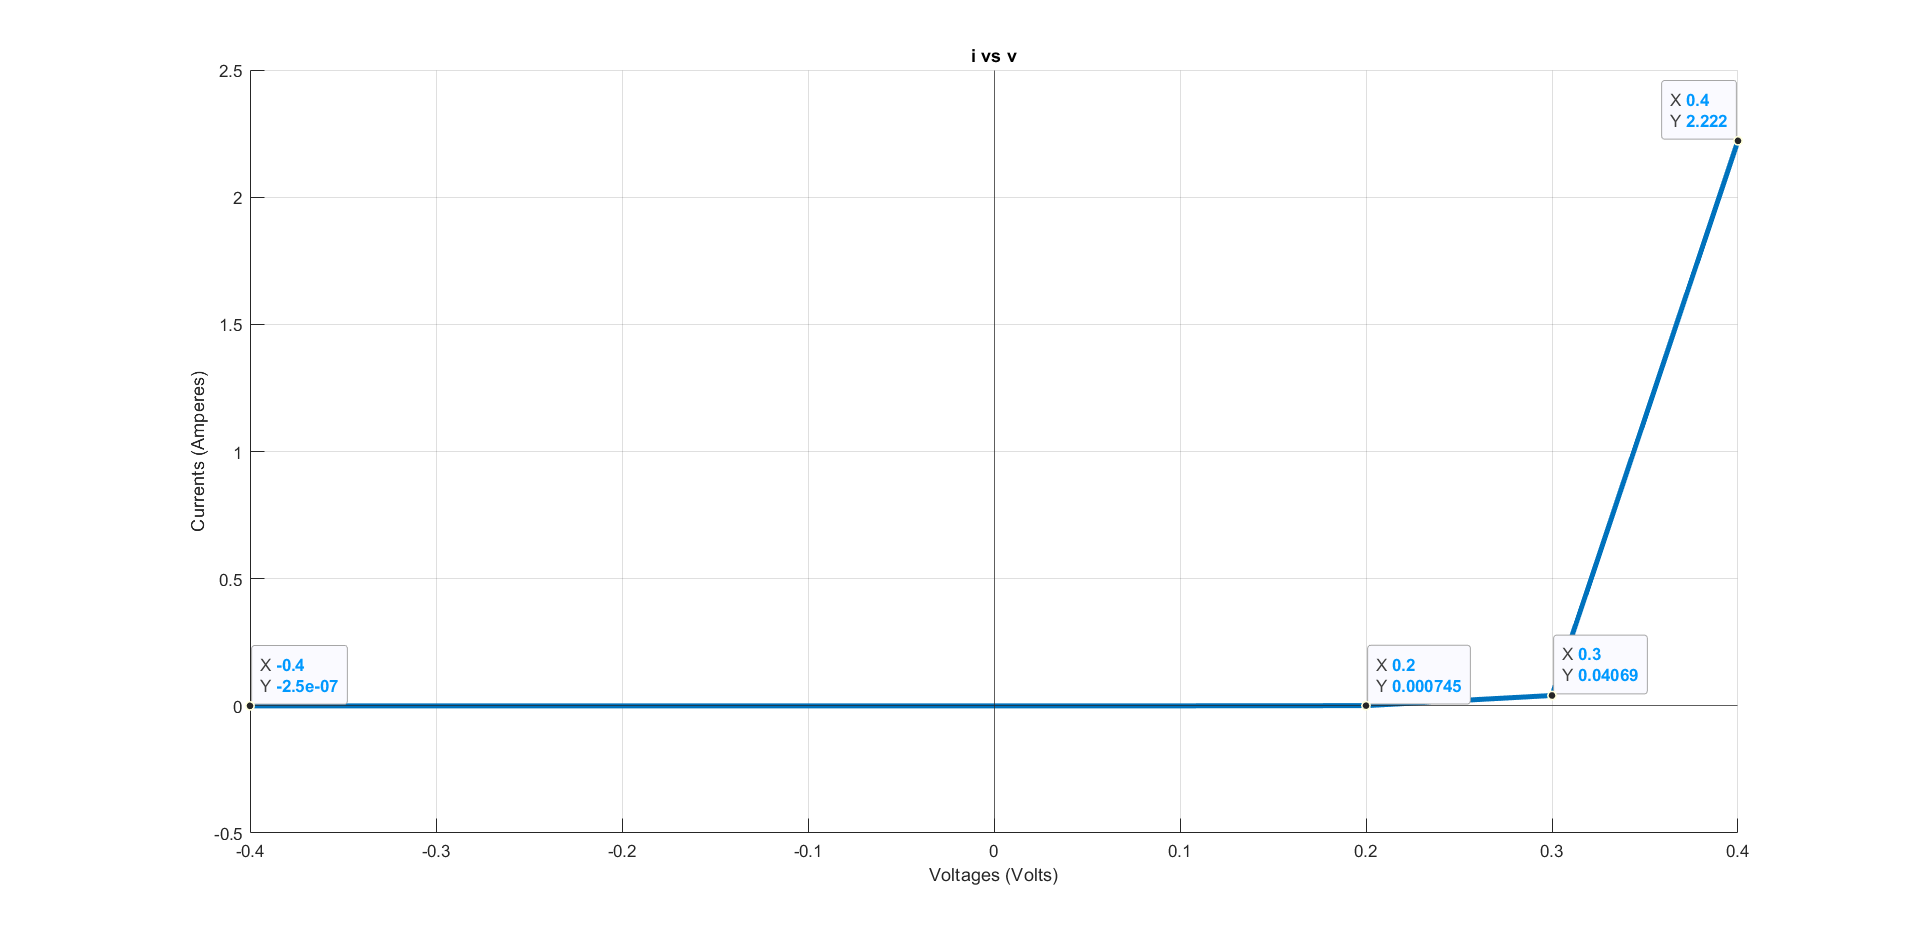
\includegraphics[width=1\textwidth]{3a.png}
\caption{i versus v plot}
\end{figure} 
    
\begin{table}[H]
    \begin{center}
    \caption{ Parameters obtained from the plot}
    \vspace{2mm}
    \begin{tabular}{||c | c | c ||} 
    \hline
    \(V_{on}\) &  \(r_f\) & \(r_r\)\\ [0.5ex] 
    \hline\hline
    0.3V & 0.046\(\Omega\)  & 2.5\(\Omega\)   \\ 
    
\hline
\end{tabular}
\end{center}
\end{table}
    

    
    
\subsection{b)}

\begin{table}[H]
\begin{center}
\caption{ I vs V}
\vspace{2mm}
\begin{tabular}{||c | c ||} 
\hline
V(Volts) & I (Amps) \\ [0.5ex] 
\hline\hline
-0.40 & -9.999998874648254e-16  \\ 
\hline
-0.20 & -9.996645373720976e-16  \\ 
\hline
0 & 0  \\ 
\hline
0.20 & 2.979957987041728e-12  \\ 
\hline
0.40 & 8.886109520507873e-09  \\ 

\hline
0.50 & 4.851651944097903e-07  \\ 
\hline
0.60 & 2.648912212884338e-05  \\ 
\hline
0.70 & 0.001446257064290  \\ 
\hline
0.80 & 0.078962960182680  \\ 
\hline
\end{tabular}
\end{center}
\end{table}



\begin{figure}[H]
    \centering
    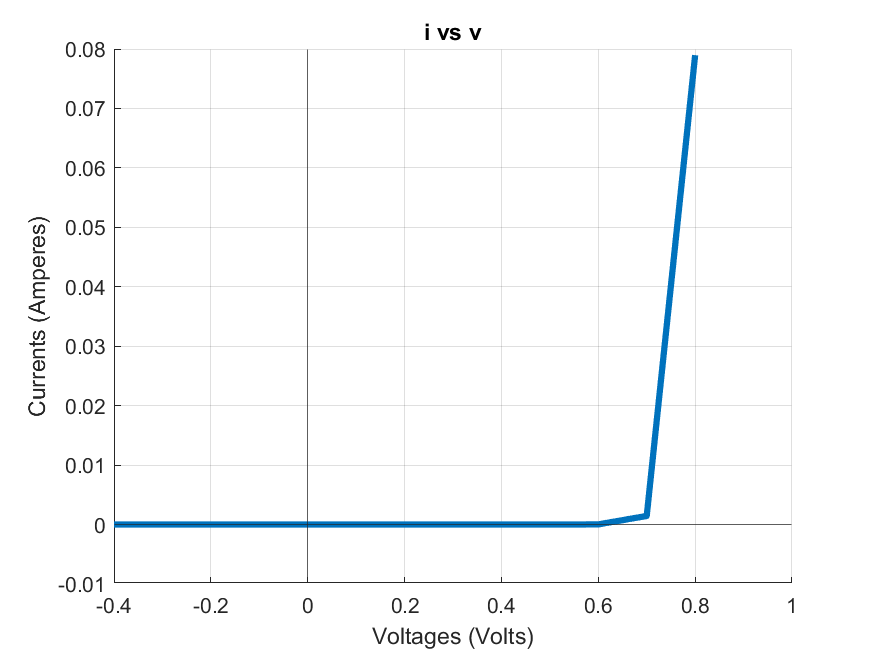
\includegraphics[width=1\textwidth]{3b.png}
    \caption{i versus v plot}
\end{figure} 
\begin{table}[H]
    \begin{center}
    \caption{ Parameters obtained from the plot}
    \vspace{2mm}
    \begin{tabular}{||c | c | c ||} 
    \hline
    \(V_{on}\) &  \(r_f\) & \(r_r\)\\ [0.5ex] 
    \hline\hline
    0.7V & 1.2893\(\Omega\)  & 68.97\(\Omega\)   \\ 
    
\hline
\end{tabular}
\end{center}
\end{table}

\section{Step 4}

%Hand

\begin{figure}[H]
    \centering
   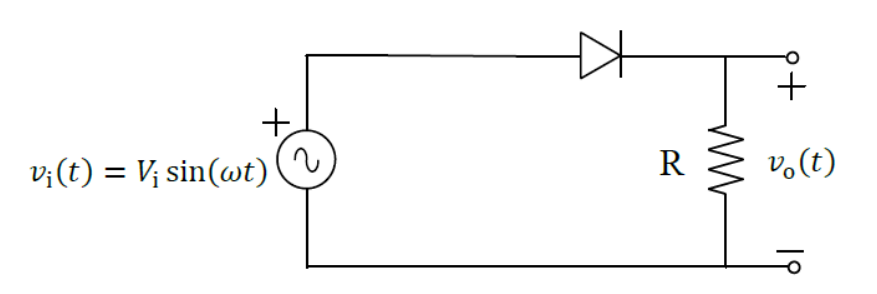
\includegraphics[width=1\textwidth]{4_1.png}
   \caption{Half-wave circuit schematic for the Step 4}
\end{figure} 

\section{Step 5}
%Hand

\begin{figure}[H]
    \centering
   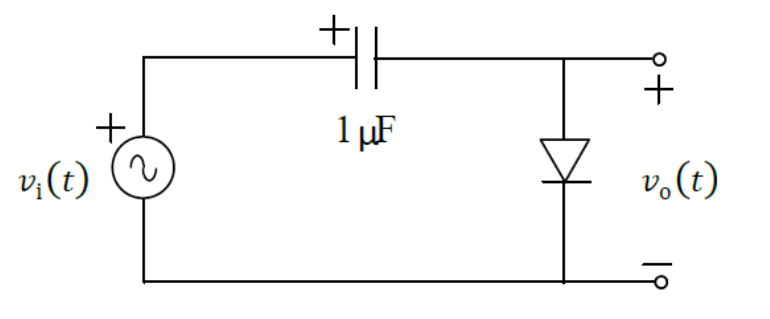
\includegraphics[width=1\textwidth]{5_1.png}
   \caption{Diode clamper circuit schematic for the Step 5}
\end{figure} 

\begin{figure}[H]
    \centering
   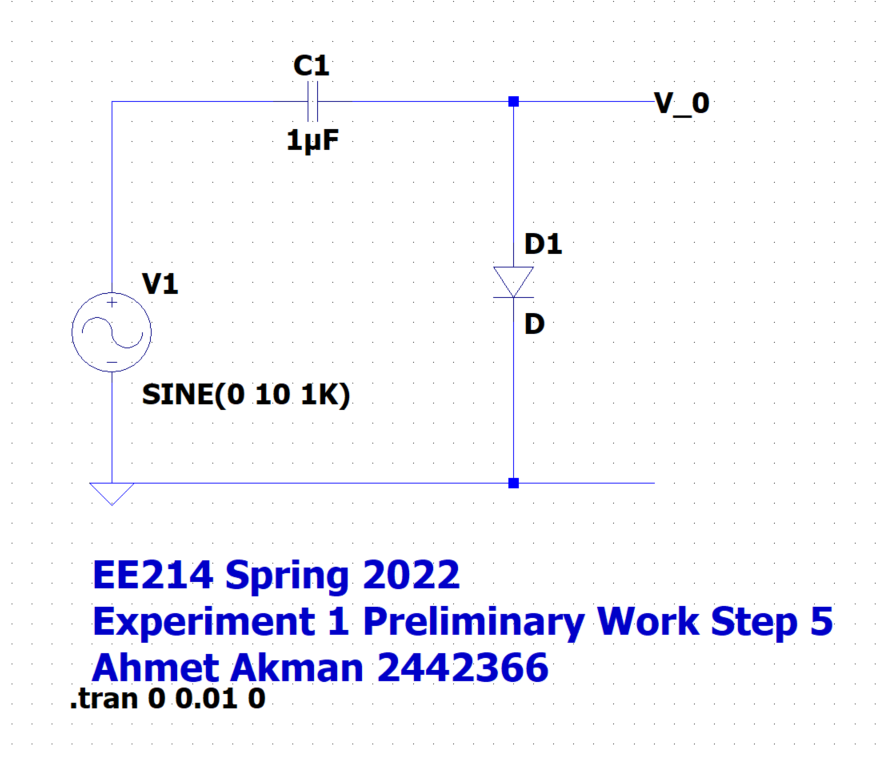
\includegraphics[width=1\textwidth]{5SCH.png}
   \caption{Diode clamper circuit simulation schematic for the Step 5}
\end{figure} 



\subsection{a)}
\begin{figure}[H]
    \centering
   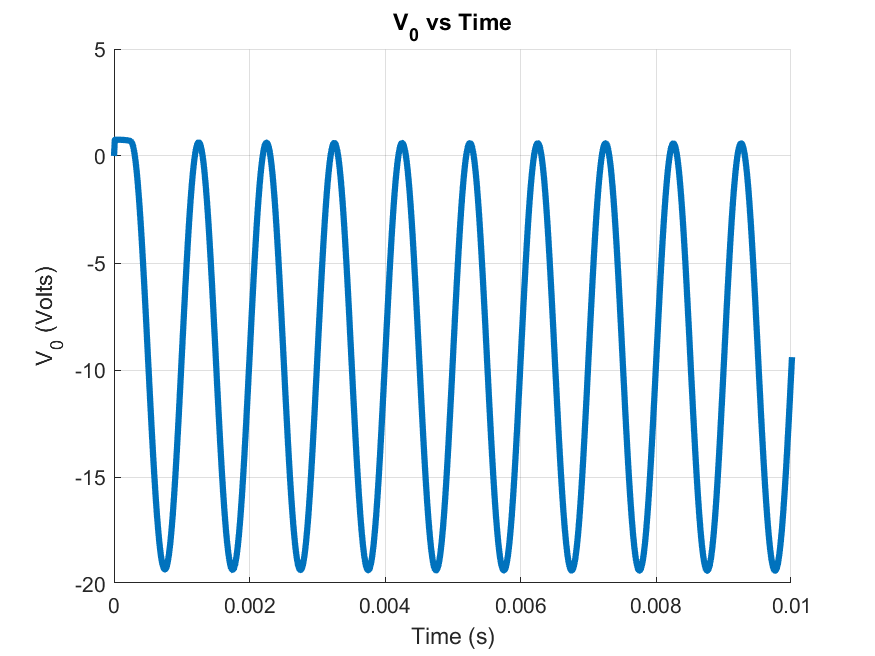
\includegraphics[width=1\textwidth]{5a.png}
   \caption{Diode clamper circuit simulation plot}
\end{figure} 
\subsection{b)}
\begin{figure}[H]
    \centering
   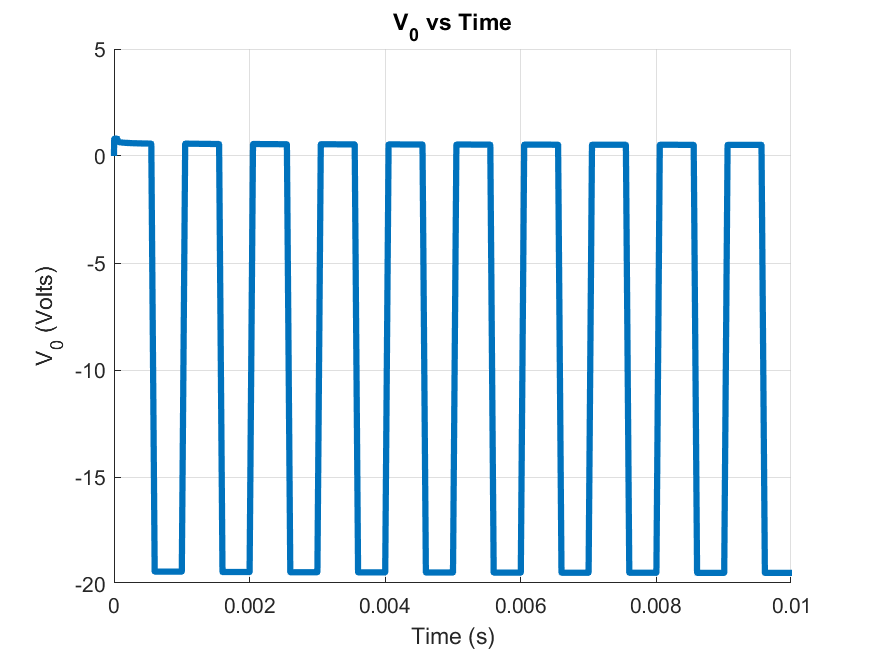
\includegraphics[width=1\textwidth]{5b.png}
   \caption{Diode clamper circuit simulation plot (Square wave input)}
\end{figure} 

\section{Step 6}

\begin{figure}[H]
    \centering
   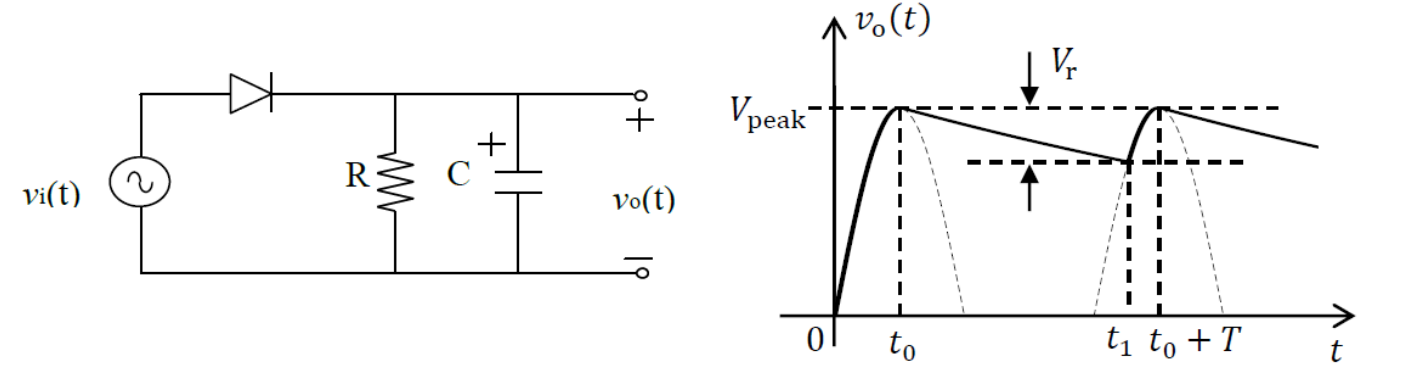
\includegraphics[width=1\textwidth]{6_1.png}
   \caption{Half-wave rectifier circuit schematic for the Step 6}
\end{figure} 


\begin{figure}[H]
    \centering
   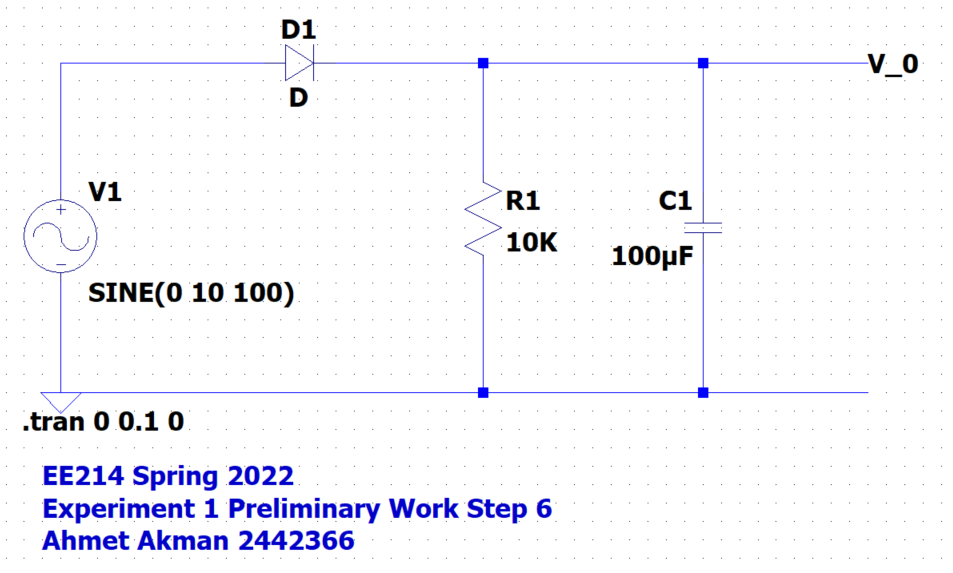
\includegraphics[width=1\textwidth]{6SCH.png}
   \caption{Half-wave rectifier circuit simulation schematic for the Step 6}
\end{figure} 



\subsection{a)}


\subsection{b)}
\begin{figure}[H]
    \centering
   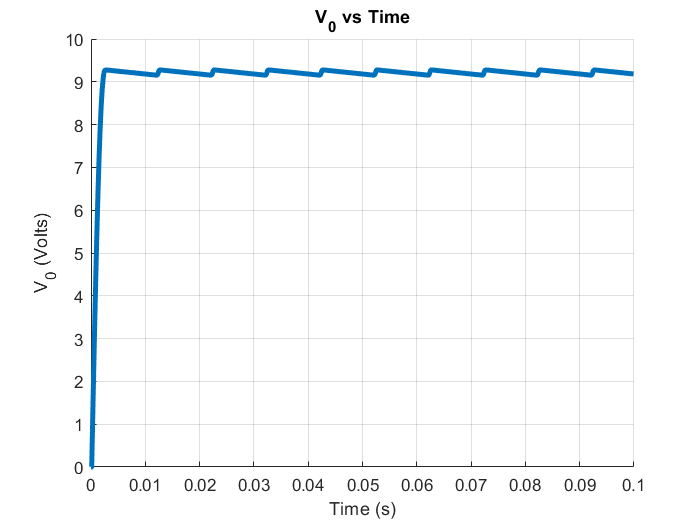
\includegraphics[width=1\textwidth]{6.png}
   \caption{Half wave rectifier circuit simulation plot \(V_o\) }
\end{figure} 
\subsection{c)}

\section{Step 7}

\begin{figure}[H]
    \centering
   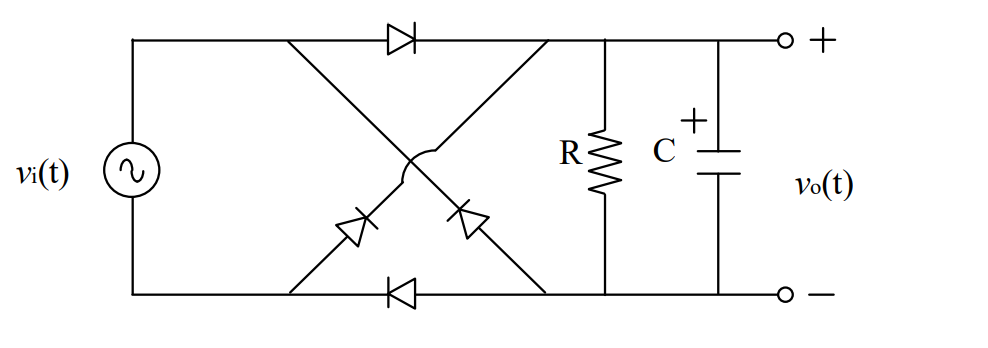
\includegraphics[width=1\textwidth]{7_1.png}
   \caption{Full-wave rectifier circuit schematic for the Step 7}
\end{figure} 


\begin{figure}[H]
    \centering
   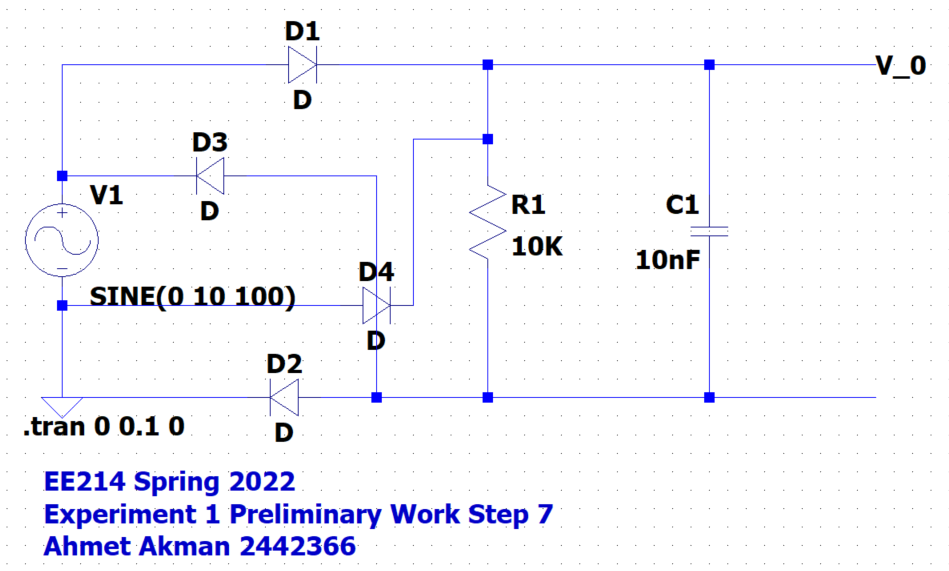
\includegraphics[width=1\textwidth]{7SCH.png}
   \caption{Full-wave rectifier circuit simulation schematic for the Step 7}
\end{figure} 

\begin{figure}[H]
    \centering
   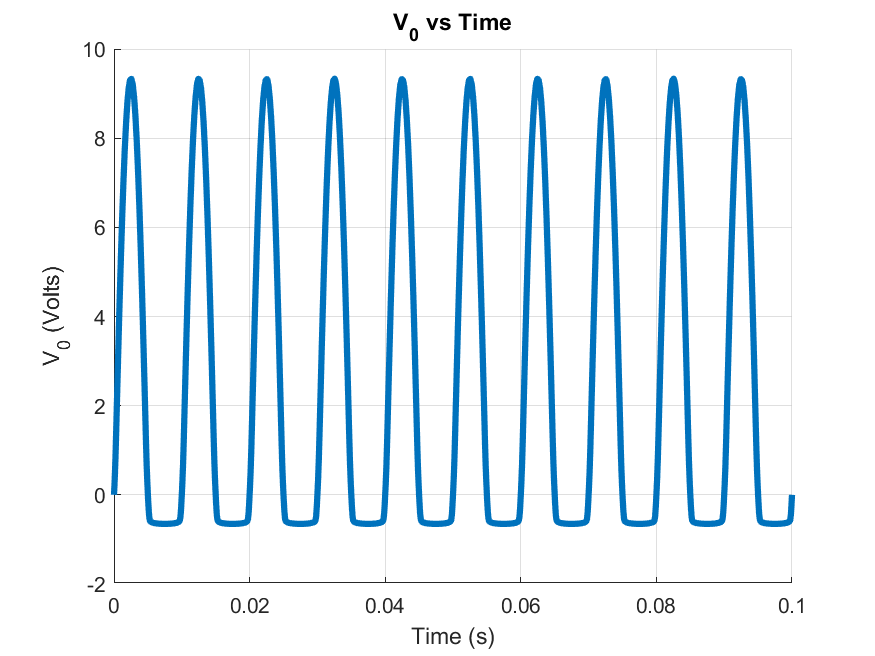
\includegraphics[width=1\textwidth]{7_empty.png}
   \caption{Full-wave rectifier circuit simulation plot \(V_o\) || no capacitor }
\end{figure} 

\begin{figure}[H]
    \centering
   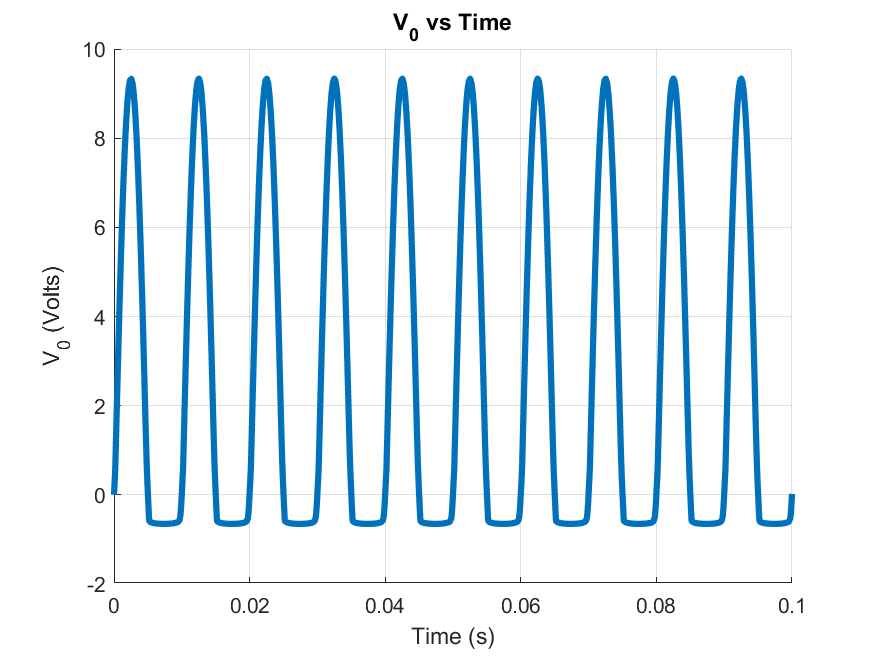
\includegraphics[width=1\textwidth]{7_10nF.png}
   \caption{Full-wave rectifier circuit simulation plot \(V_o\) || 10nF capacitor}
\end{figure} 



\begin{figure}[H]
    \centering
   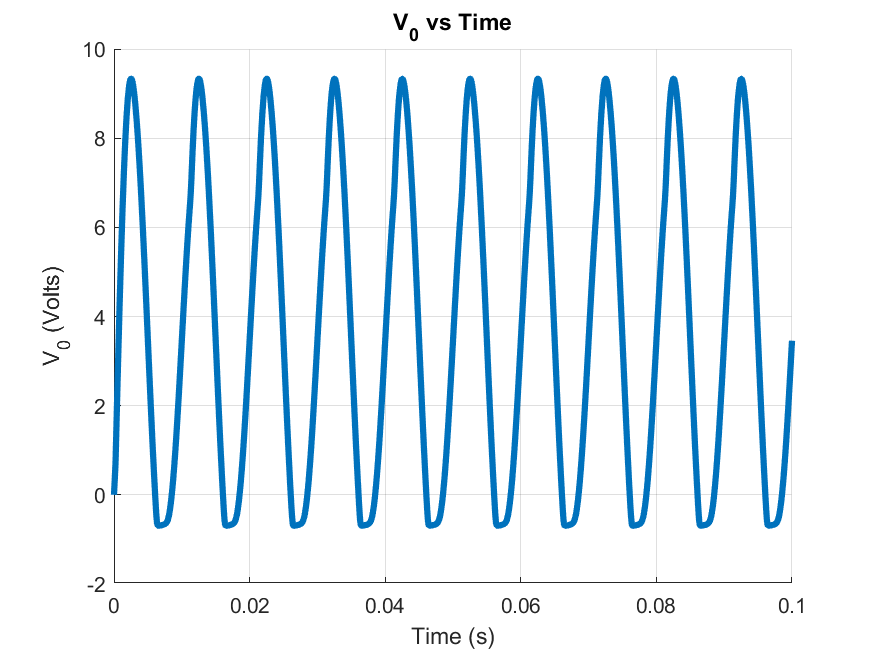
\includegraphics[width=1\textwidth]{7_1uF.png}
   \caption{Full-wave rectifier circuit simulation plot \(V_o\) || 1uF capacitor }
\end{figure} 




\section{Step 8}
%LTSpice

\begin{figure}[H]
    \centering
   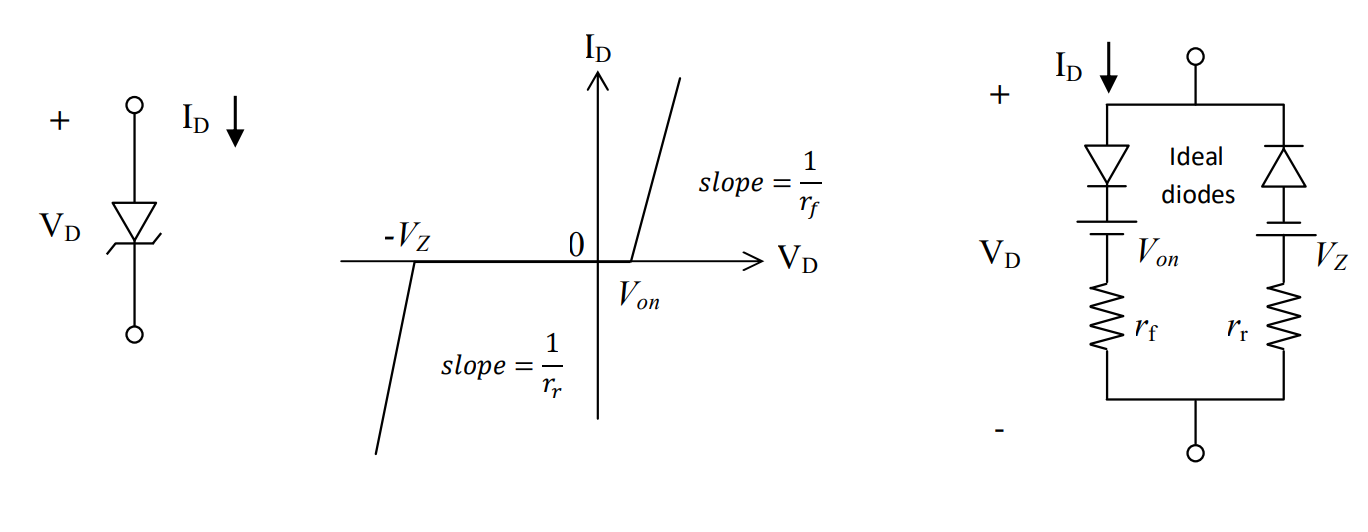
\includegraphics[width=1\textwidth]{8_1.png}
   \caption{Common piecewise linear model for a zener diode.}
\end{figure} 


\begin{table}[H]
    \begin{center}
    \caption{ Parameters from datasheet}
    \vspace{2mm}
    \begin{tabular}{||c | c ||} 
    \hline
    Parameter & Value \\ [0.5ex] 
    \hline\hline
    \(V_{on}\) & 0.5V  \\ 
    \hline
    \(V_z\) & 6.2V  \\ 
    \hline
    \(r_f\) & 0.003 \(\Omega\)  \\ 
    \hline
    \(r_r\)& 1 to 10 \(\Omega\)  \\ 
\hline
\end{tabular}
\end{center}
\end{table}


\section{Step 9}
%LTSpice
\begin{figure}[H]
    \centering
   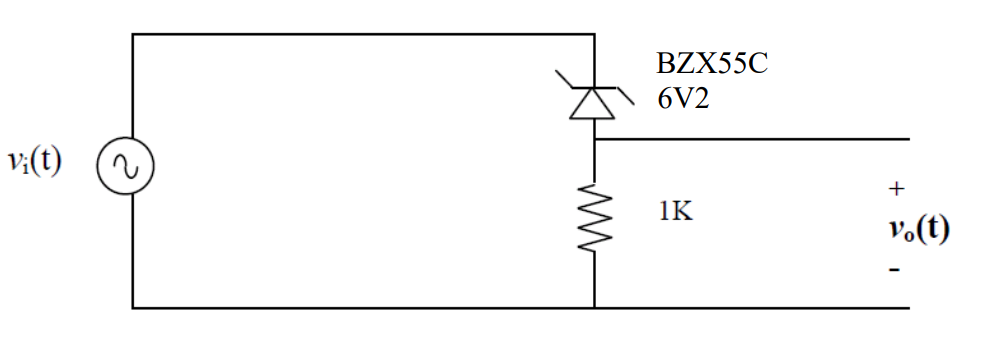
\includegraphics[width=1\textwidth]{9_1.png}
   \caption{DC level shifter circuit schematic for the Step 9}
\end{figure} 


\begin{figure}[H]
    \centering
   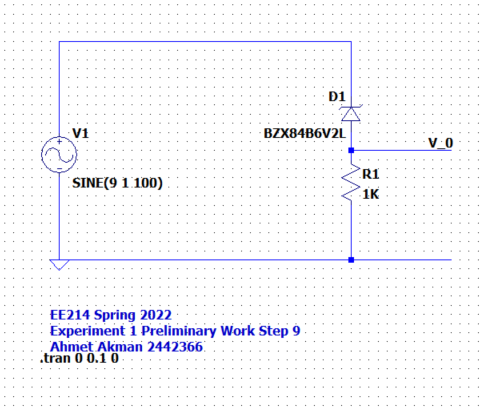
\includegraphics[width=1\textwidth]{9SCH.png}
   \caption{DC level shifter circuit simulation schematic for the Step 9}
\end{figure} 

\begin{figure}[H]
    \centering
   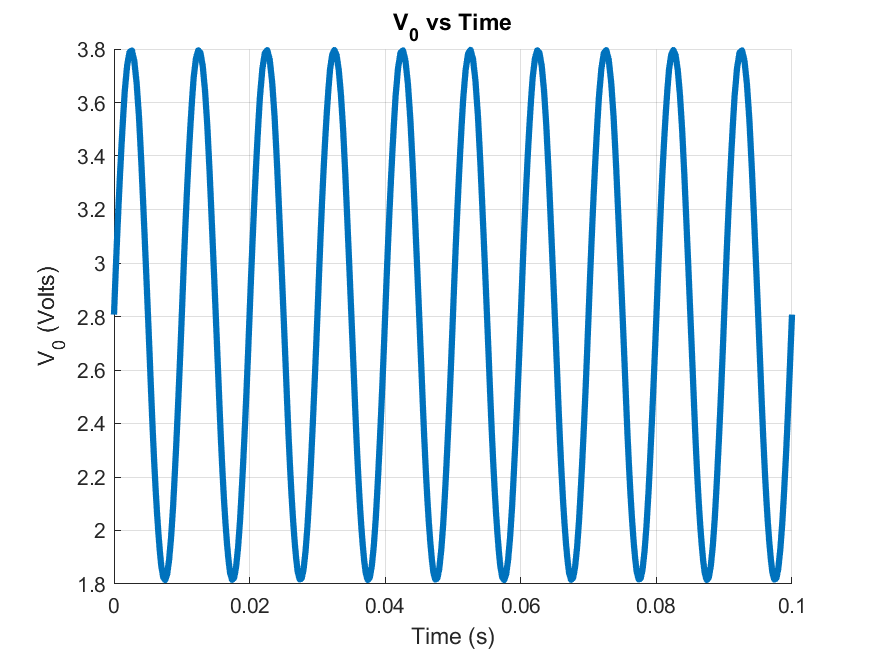
\includegraphics[width=1\textwidth]{9.png}
   \caption{DC level shifter circuit simulation  plot \(V_o\)}
\end{figure} 

\section{Step 10}
%LTSpice
\begin{figure}[H]
    \centering
   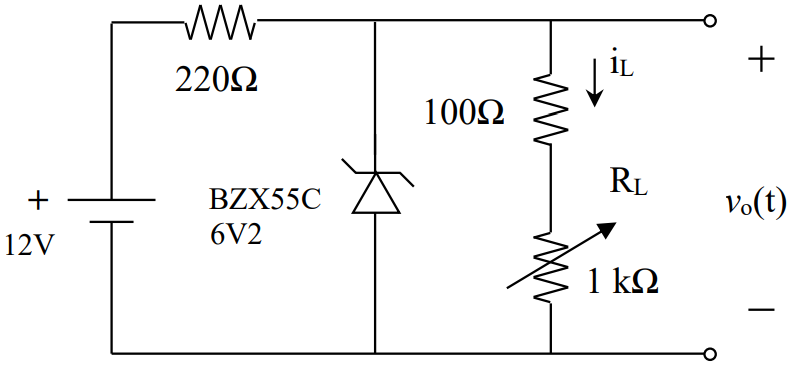
\includegraphics[width=1\textwidth]{10_1.png}
   \caption{Regulation with zener diode circuit schematic for the Step 10}
\end{figure} 

\begin{figure}[H]
    \centering
   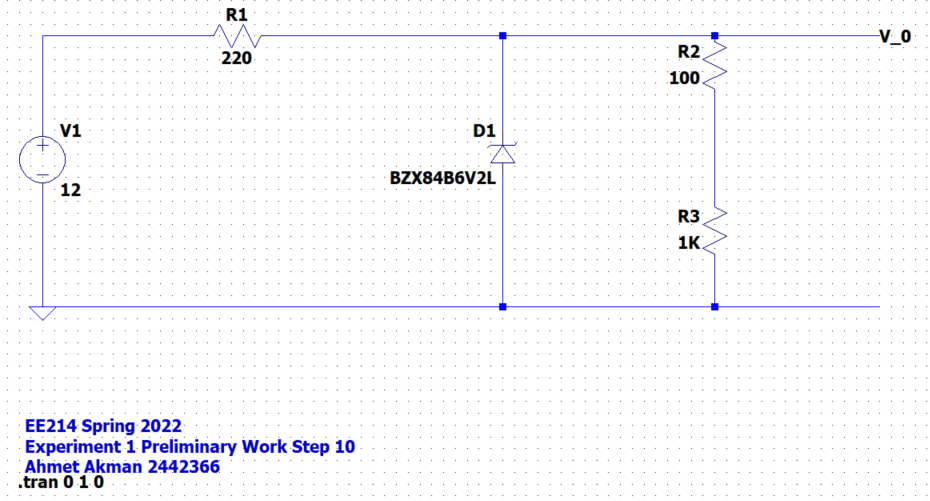
\includegraphics[width=1\textwidth]{10SCH.png}
   \caption{Regulation with zener diode circuit simulation schematic for the Step 10}
\end{figure} 


\section{Step 11}
%LTSpice
\begin{figure}[H]
    \centering
   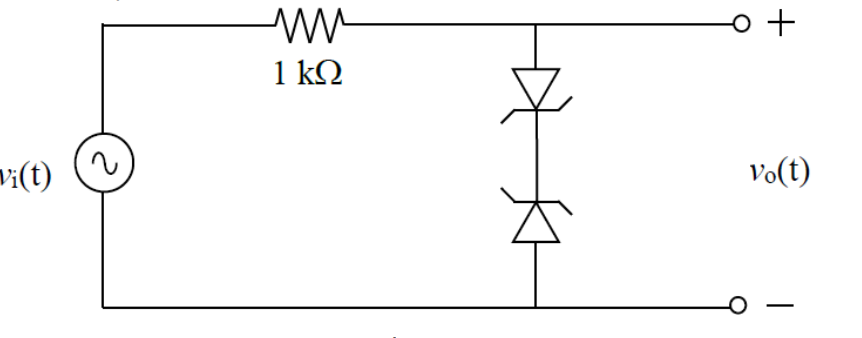
\includegraphics[width=1\textwidth]{11_1.png}
   \caption{Clipper circuit schematic for the Step 11}
\end{figure} 


\begin{figure}[H]
\centering
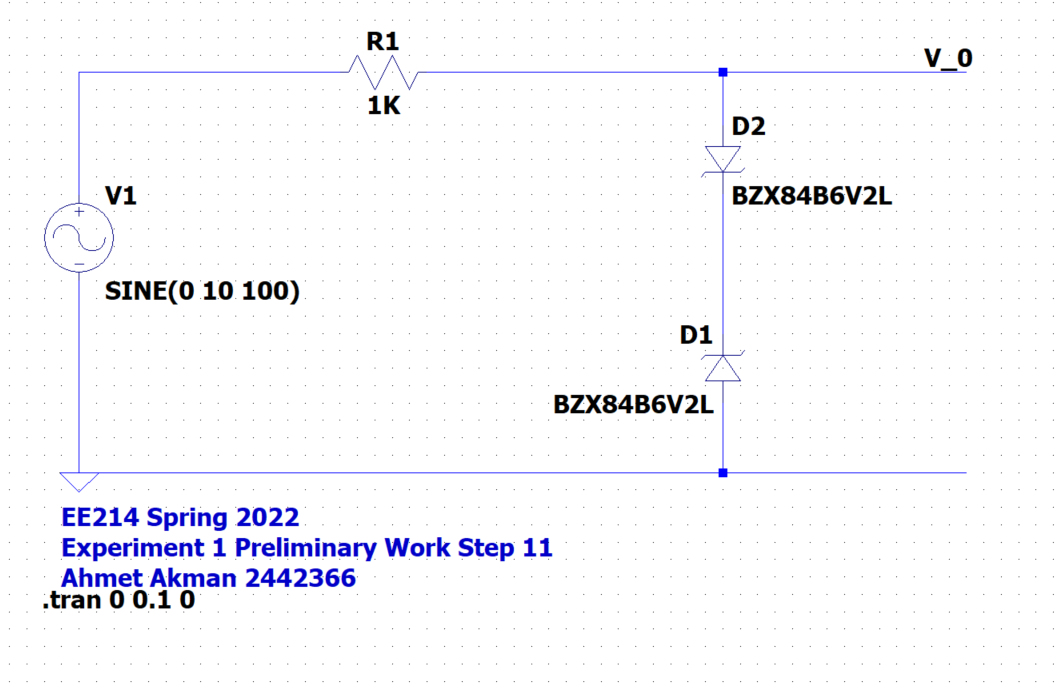
\includegraphics[width=1\textwidth]{11SCH.png}
\caption{Clipper circuit simulation schematic for the Step 11}
\end{figure} 



\begin{figure}[H]
    \centering
   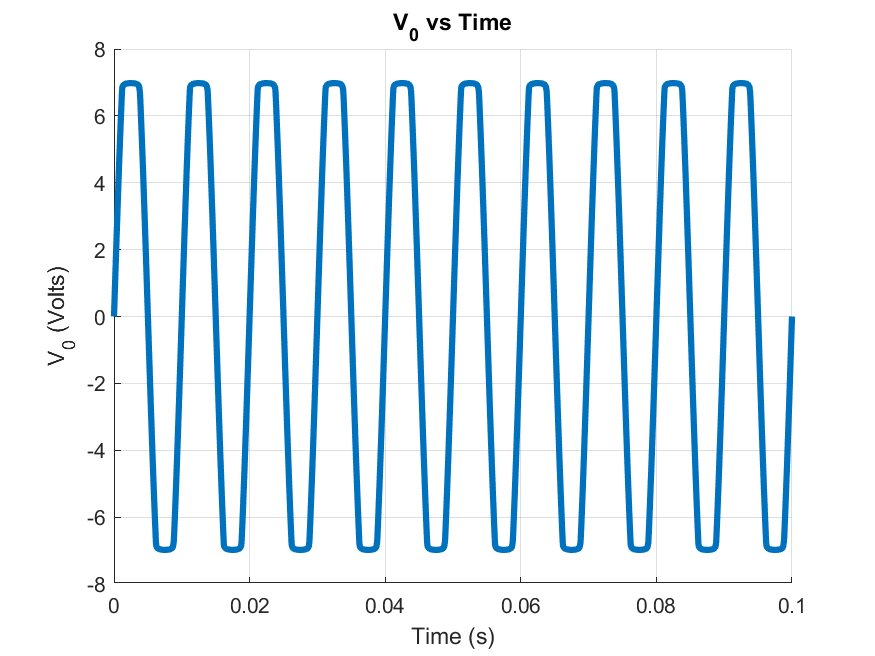
\includegraphics[width=1\textwidth]{11.png}
   \caption{Clipper circuit simulation plot \(V_o\) }
\end{figure} 

\iffalse
\section{Step 12}
%LTSpice and BONUS

\subsection{a)}
\begin{figure}[H]
    \centering
   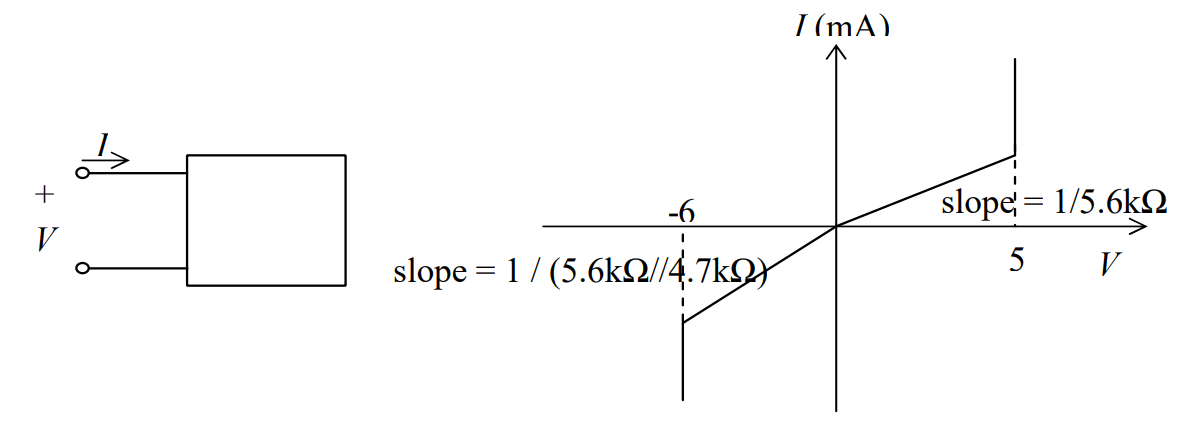
\includegraphics[width=1\textwidth]{12_1.png}
   \caption{i-v characteristics of a box for the Step 12 part a}
\end{figure} 

\subsection{b)}
\begin{figure}[H]
    \centering
   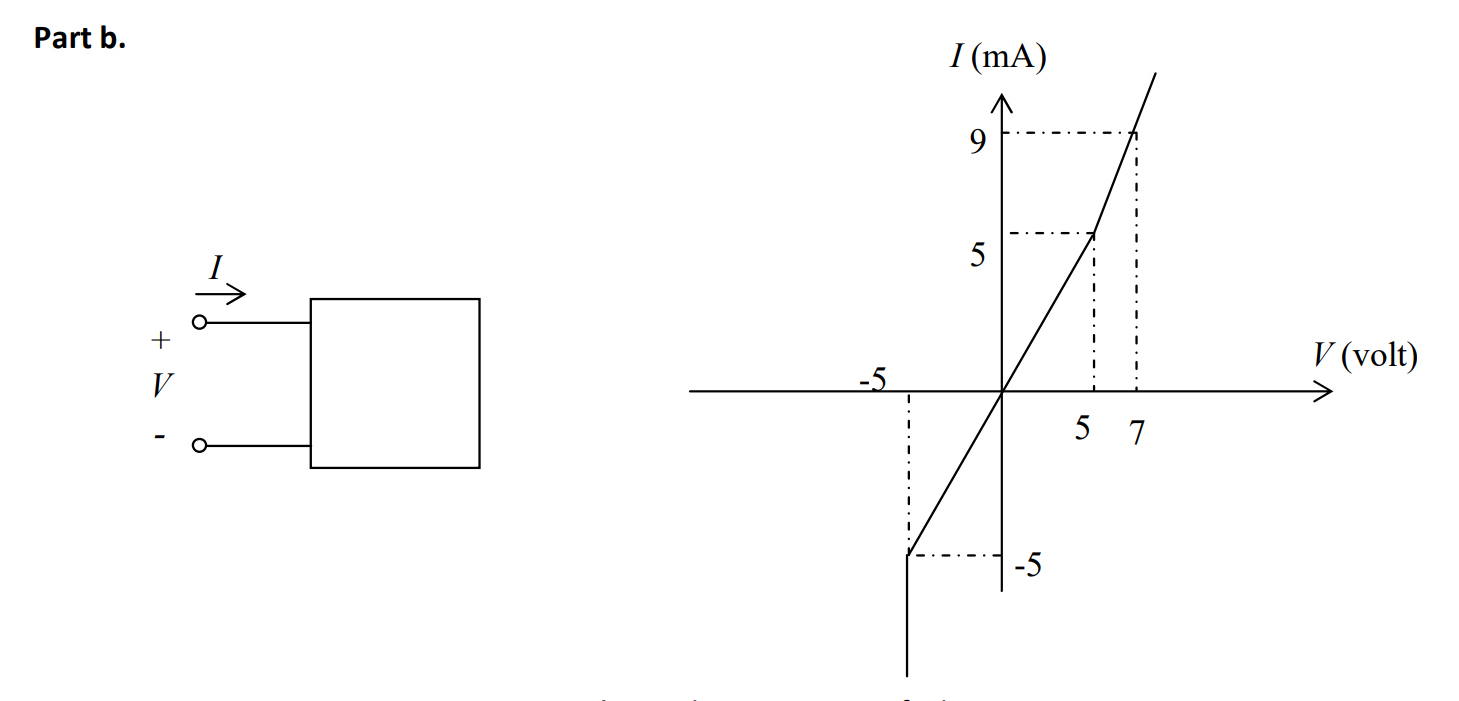
\includegraphics[width=1\textwidth]{12_2.png}
   \caption{i-v characteristics of a box for the Step 12 part b}
\end{figure} 
\fi
\section{Conclusion}


\end{document}

%%%%%%%%%%%%%%%%%%%%%%   EXAMPLE TABLE   %%%%%%%%%%%%%%%%%%%%%%%%%%%%%%%%
\begin{table}[H]
\begin{center}
    \caption{Resistance reading by color code convention.}
    \vspace{2mm}
    \begin{tabular}{||c | c | c||} 
        \hline
        Color Order & Value & Tolerance \\ [0.5ex] 
        \hline\hline
        Brown / Black / Red / Gold & 1k\( \Omega \) & \( \% \) 5  \\ 
        \hline
        Yellow / Violet / Red / Gold & 4.7k\( \Omega \) & \( \% \) 5   \\
        \hline
        Brown / Grey / Orange / Gold & 18k\( \Omega \) & \( \% \) 5  \\ [1ex] 
        \hline
    \end{tabular}
\end{center}
\end{table}


%%%%%%%%%%%%%%%%%%%%%%   EXAMPLE IMAGE   %%%%%%%%%%%%%%%%%%%%%%%%%%%%%%%%
\begin{figure}[H]
\centering
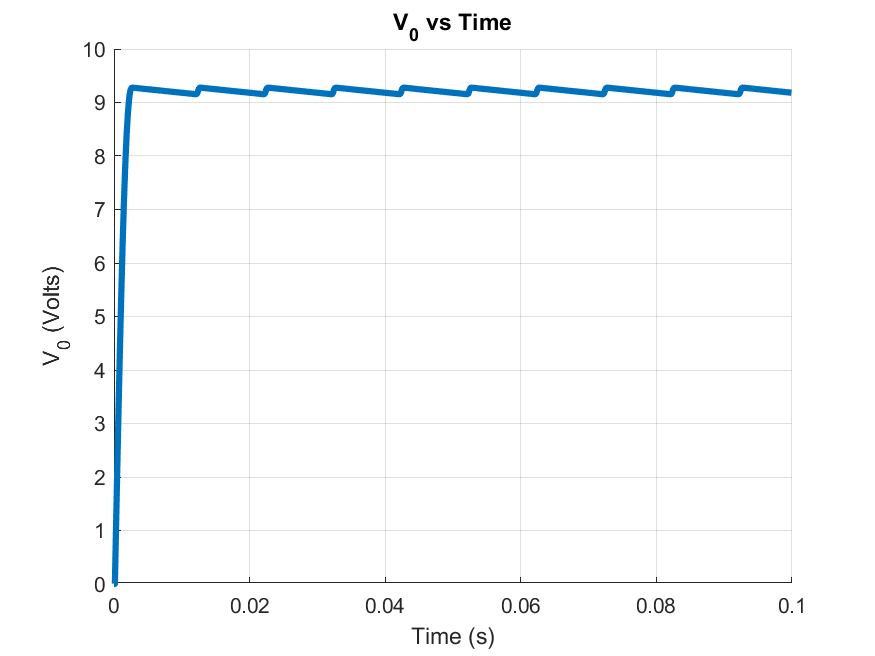
\includegraphics[width=1\textwidth]{5.png}
\caption{Circuit schematic for the step 5}
\end{figure} 

%%%%%%%%%%%%%%%%%%%%%%   EXAMPLE IMAGE FROM PDF   %%%%%%%%%%%%%%%%%%%%%%%%%%%%%%%%
\begin{figure}[H] \centering{
	\includegraphics[scale=0.25]{2a_plot.pdf}}
	\caption{Experiment 2}
\end{figure}
	